\section{The Task}
	\label{sec-workflow-task}
	To illustrate how \emph{q2d} can be used productively, consider the following workflow example.
	For this purpose, a \gls{clb} as it is used in \textsc{Xilinx Virtex 5} \glspl{fpga} is to be modelled.
	A circuit diagram of the part in question is given in figure \ref{fig-clb-detail}.
	More information regarding the actual architecture can be found in the official manual.\footnote{
		Available at \url{www.xilinx.com/support/documentation/user_guides/ug190.pdf}
	}\cite{virtex5}
	Further, the configuration required to realize a \emph{full adder} with this model shall be computed.

	\begin{figure}[p]
	\centering
		\resizebox{0.9\textwidth}{!}{
		
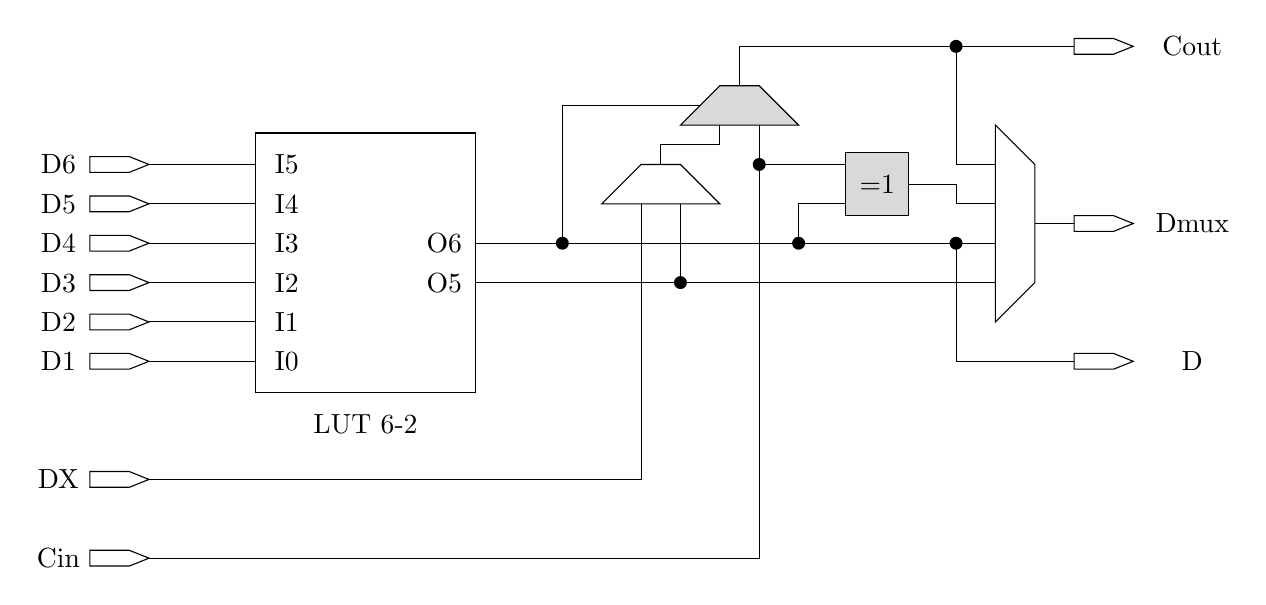
\begin{tikzpicture}

% inputs
\draw (0mm, -1mm) -- (5mm, -1mm) -- (7.5mm, 0mm) -- (5mm, 1mm) -- (0mm, 1mm) -- cycle;
\draw (0mm, 4mm) -- (5mm, 4mm) -- (7.5mm, 5mm) -- (5mm, 6mm) -- (0mm, 6mm) -- cycle;
\draw (0mm, 9mm) -- (5mm, 9mm) -- (7.5mm, 10mm) -- (5mm, 11mm) -- (0mm, 11mm) -- cycle;
\draw (0mm, 14mm) -- (5mm, 14mm) -- (7.5mm, 15mm) -- (5mm, 16mm) -- (0mm, 16mm) -- cycle;
\draw (0mm, 19mm) -- (5mm, 19mm) -- (7.5mm, 20mm) -- (5mm, 21mm) -- (0mm, 21mm) -- cycle;
\draw (0mm, 24mm) -- (5mm, 24mm) -- (7.5mm, 25mm) -- (5mm, 26mm) -- (0mm, 26mm) -- cycle;

\draw (-4mm, 0mm) node {D1};
\draw (-4mm, 5mm) node {D2};
\draw (-4mm, 10mm) node {D3};
\draw (-4mm, 15mm) node {D4};
\draw (-4mm, 20mm) node {D5};
\draw (-4mm, 25mm) node {D6};

% lut
\draw (25mm, 0mm) node {I0};
\draw (25mm, 5mm) node {I1};
\draw (25mm, 10mm) node {I2};
\draw (25mm, 15mm) node {I3};
\draw (25mm, 20mm) node {I4};
\draw (25mm, 25mm) node {I5};

\draw (45mm, 10mm) node {O5};
\draw (45mm, 15mm) node {O6};
\draw(35mm, -8mm) node{LUT 6-2};

\draw(21mm, -4mm) rectangle (49mm, 29mm);

% dx
\draw (0mm, -16mm) -- (5mm, -16mm) -- (7.5mm, -15mm) -- (5mm, -14mm) -- (0mm, -14mm) -- cycle;
\draw (-4mm, -15mm) node {DX};

% cin
\draw (0mm, -26mm) -- (5mm, -26mm) -- (7.5mm, -25mm) -- (5mm, -24mm) -- (0mm, -24mm) -- cycle;
\draw (-4mm, -25mm) node {Cin};

% mux
\draw[fill=gray!30!white](75mm, 30mm) -- (90mm, 30mm) -- (85mm, 35mm) -- (80mm, 35mm) -- cycle;

% cmux
\draw(65mm, 20mm) -- (80mm, 20mm) -- (75mm, 25mm) -- (70mm, 25mm) -- cycle;

% xor
\draw[fill=gray!30!white](96mm, 18.5mm) rectangle (104mm, 26.5mm);
\draw(100mm, 22.5mm) node{=1};

% cmux-d
\draw(115mm, 5mm) -- (120mm, 10mm) -- (120mm, 25mm) -- (115mm, 30mm) -- cycle;

%cout
\draw (125mm, 39mm) -- (130mm, 39mm) -- (132.5mm, 40mm) -- (130mm, 41mm) -- (125mm, 41mm) -- cycle;
\draw (140mm, 40mm) node {Cout};

%dmux
\draw (125mm, 16.5mm) -- (130mm, 16.5mm) -- (132.5mm, 17.5mm) -- (130mm, 18.5mm) -- (125mm, 18.5mm) -- cycle;
\draw (140mm, 17.5mm) node {Dmux};

%d
\draw (125mm, -1mm) -- (130mm, -1mm) -- (132.5mm, 0mm) -- (130mm, 1mm) -- (125mm, 1mm) -- cycle;
\draw (140mm, 0mm) node {D};

% wiring
	% inputs -> lut
\draw(7.5mm, 0mm) -- (21mm, 0mm);
\draw(7.5mm, 5mm) -- (21mm, 5mm);
\draw(7.5mm, 10mm) -- (21mm, 10mm);
\draw(7.5mm, 15mm) -- (21mm, 15mm);
\draw(7.5mm, 20mm) -- (21mm, 20mm);
\draw(7.5mm, 25mm) -- (21mm, 25mm);
	% O5 ->cmux
\draw[fill] (75mm, 10mm) circle (.75mm);
\draw(49mm, 10mm) -- (75mm, 10mm) -- (75mm, 20mm);
	% DX ->cmux
\draw(7.5mm, -15mm) -- (70mm, -15mm) -- (70mm, 20mm);
	% cmux -> mux
\draw(72.5mm, 25mm) -- (72.5mm, 27.5mm) -- (80mm, 27.5mm) -- (80mm, 30mm);
	% cim -> mux
\draw(7.5mm, -25mm) -- (85mm, -25mm) -- (85mm, 30mm);
	% O6 -> mux
\draw[fill](60mm, 15mm) circle (.75mm);
\draw(49mm, 15mm) -- (60mm, 15mm) -- (60mm, 32.5mm) -- (77.5mm, 32.5mm);
	% O6 -> xor
\draw[fill](90mm, 15mm) circle (.75mm);
\draw(60mm, 15mm) -- (90mm, 15mm) -- (90mm, 20mm) -- (96mm, 20mm);
	% Cin -> xor
\draw[fill](85mm, 25mm) circle (.75mm);
\draw(85mm, 25mm) -- (96mm, 25mm);
	% O5 -> cmux-d
\draw(75mm, 10mm) -- (115mm, 10mm);
	% O6 -> cmux-d
\draw(90mm, 15mm) -- (115mm, 15mm);
	% xor -> cmux-d
\draw(104mm, 22.5mm) -- (110mm, 22.5mm) -- (110mm, 20mm) -- (115mm, 20mm);
	% mux -> cout
\draw(82.5mm, 35mm) -- (82.5mm, 40mm) -- (125mm, 40mm);
	%mux ->cmux-d
\draw[fill](110mm, 40mm) circle (.75mm);
\draw(110mm, 40mm) -- (110mm, 25mm) -- (115mm, 25mm);
	%O6 -> d
\draw[fill](110mm, 15mm) circle (.75mm);
\draw(110mm, 15mm) -- (110mm, 0mm) -- (125mm, 0mm);
	% cmux-d ->dmux
\draw(120mm, 17.5mm) -- (125mm, 17.5mm);
\end{tikzpicture}
		}
		\caption{Circuit Diagram of a CLB Detail}
		White components are configurable.
		\label{fig-clb-detail}
	\end{figure}		

	\begin{figure}[p]
	\centering
		\resizebox{!}{0.4\textheight}{
		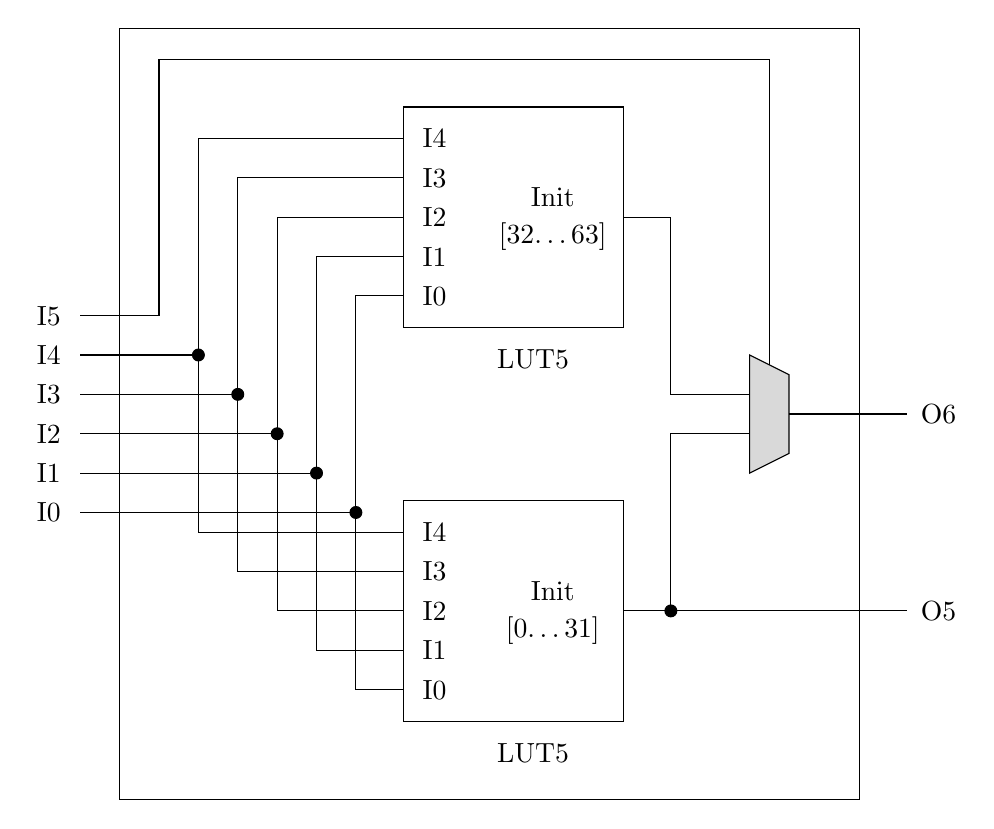
\begin{tikzpicture}

%lut6
\draw(-30mm, -49mm) rectangle (64mm, 49mm);
\draw(-39mm, 12.5mm) node{I5};
\draw(-39mm, 7.5mm) node{I4};
\draw(-39mm, 2.5mm) node{I3};
\draw(-39mm, -2.5mm) node{I2};
\draw(-39mm, -7.5mm) node{I1};
\draw(-39mm, -12.5mm) node{I0};

\draw(74mm, 0mm) node{O6};
\draw(74mm, -25mm) node{O5};

% lut1
\draw(6mm, 11mm) rectangle (34mm, 39mm);
\draw(10mm, 35mm) node{I4};
\draw(10mm, 30mm) node{I3};
\draw(10mm, 25mm) node{I2};
\draw(10mm, 20mm) node{I1};
\draw(10mm, 15mm) node{I0};

\draw(22.5mm, 7mm) node {LUT5};

\draw(25mm, 27.5mm) node {Init};
\draw(25mm, 22.5mm) node {[32\dots63]};

% lut2
\draw(6mm, -11mm) rectangle (34mm, -39mm);
\draw(10mm, -15mm) node{I4};
\draw(10mm, -20mm) node{I3};
\draw(10mm, -25mm) node{I2};
\draw(10mm, -30mm) node{I1};
\draw(10mm, -35mm) node{I0};

\draw(22.5mm, -43mm) node {LUT5};

\draw(25mm, -22.5mm) node {Init};
\draw(25mm, -27.5mm) node {[0\dots31]};

%cmux
\draw[fill=gray!30!white](50mm, 7.5mm) -- (50mm, -7.5mm) -- (55mm, -5mm) -- (55mm, 5mm) -- cycle;

%wiring
	%lut1 -> cmux
\draw(34mm, 25mm) -- (40mm, 25mm) -- (40mm, 2.5mm) -- (50mm, 2.5mm);
	%lut2 -> cmux
\draw(34mm, -25mm) -- (40mm, -25mm) -- (40mm, -2.5mm) -- (50mm, -2.5mm);

	%I0
\draw(-35mm, -12.5mm) -- (0mm, -12.5mm) -- (0mm, -35mm) -- (6mm, -35mm);
\draw[fill](0mm, -12.5mm) circle (0.75mm);
\draw(0mm, -12.5mm) -- (0mm, 15mm) --(6mm, 15mm);

	%I1
\draw(-35mm, -7.5mm) -- (-5mm, -7.5mm) -- (-5mm, -30mm) -- (6mm, -30mm);
\draw[fill](-5mm, -7.5mm) circle (0.75mm);
\draw(-5mm, -7.5mm) -- (-5mm, 20mm) --(6mm, 20mm);

	%I2
\draw(-35mm, -2.5mm) -- (-10mm, -2.5mm) -- (-10mm, -25mm) -- (6mm, -25mm);
\draw[fill](-10mm, -2.5mm) circle (0.75mm);
\draw(-10mm, -2.5mm) -- (-10mm, 25mm) --(6mm, 25mm);

	%I3
\draw(-35mm, 2.5mm) -- (-15mm, 2.5mm) -- (-15mm, -20mm) -- (6mm, -20mm);
\draw[fill](-15mm, 2.5mm) circle (0.75mm);
\draw(-15mm, -2.5mm) -- (-15mm, 30mm) --(6mm, 30mm);

	%I4
\draw(-35mm, 7.5mm) -- (-20mm, 7.5mm) -- (-20mm, -15mm) -- (6mm, -15mm);
\draw[fill](-20mm, 7.5mm) circle (0.75mm);
\draw(-20mm, 7.5mm) -- (-20mm, 35mm) --(6mm, 35mm);

	%I5
\draw(-35mm, 12.5mm) -- (-25mm, 12.5mm) -- (-25mm, 45mm) -- (52.5mm, 45mm) -- (52.5mm, 6.25mm);

	%O5
\draw(40mm, -25mm) -- (70mm, -25mm);
\draw[fill](40mm, -25mm) circle (0.75mm);

	%O6
\draw(55mm, 0mm) -- (70mm, 0mm);


\end{tikzpicture}


		}
		\caption{Circuit Diagram of Xilinx' LUT6-2 }
		\label{fig-lut}
	\end{figure}		

	\paragraph{How the Full Adder Will Work}
	When looking at the architecture, it is easy to see that it already provides a carry chain, which shall be used.
	The \texttt{Dmux} output will be used for the sum, which requires the \texttt{O6} port of the \gls{lut} to emit the propagate bit.
	It is notable, that the \texttt{D} output is directly attached to the respective wire, so it could be used as a proxy for the propagate bit.
	If the adder does not propagate, \texttt{Cout} will assume the value of the generate bit, which in turn has to be emitted by the port \texttt{O5}.
	Due to the \gls{lut}'s outputs having to assume different values, it is necessary to pin the input \texttt{D6} to \emph{true}, as can be inferred from the description given in section \ref{sec-xilinx-lut}.

\section{A Component Descriptor for Xilinx' LUT6-2}
	\label{sec-xilinx-lut}
	While multiplexers are not very complicated and very obvious to describe via a formula, the \gls{lut} deserves a closer look.
	A special variant, featuring six input ports, but only two output ports is employed here.
	Research of the actual components internals yields that it is composited from two 5-input \glspl{lut}.
	The sixth input determines whether both output ports will emit the same signal as determined by the lower \gls{lut} or different signals, originating from both \glspl{lut} independently. 
	This is depicted in figure \ref{fig-lut}, which also can be found in most of the official design guidelines\footnote{
		For example at \url{www.xilinx.com/support/documentation/sw_manuals/xilinx14_7/virtex5_hdl.pdf}	
	}\cite{hdl-guide}.
	Since no appropriate component descriptor for this type of \gls{lut} is commonly available yet, it has to be created from scratch.
	As outlined in section \ref{sec-user-defined-components}, this can be done even with a simple text editor.
	The resulting descriptor file is to be found in listing \ref{code-lut62-descriptor}.
	For overview reasons, the \texttt{functions} section has been shortened. 
	Since the clauses used as \glspl{pcbd} are very repetitive and systematic, users with some programming skills will most likely write a simple script to generate these lines.
	It can also be noted that there are different possible ways of describing the components behaviour correctly.
	
		\includecode[json]{sources/xi-lut6-2.json}{The Component Descriptor for Xilinx' LUT6\_2}{code-lut62-descriptor}

\section{Designing the Model}
	With all preparations made, it is simple to create the circuit within \emph{q2d}.
	In the following, a brief walk-through will be given.
	It will be assumed that a new project had been created and the current document is empty.
	
	\paragraph{Loading the Required Component Descriptors}
	Users, who start with a fresh copy of the application will most likely not yet have a set of components to choose from.
	They may either create the required component descriptors by themselves\footnote{
		Which is a great opportunity to get familiar with the component creation process.
	} or obtain such descriptors from separate sources\footnote{
		A collection of component descriptors can be found at \url{github.com/fer-rum/q2d-components}. 	
	}.
	The actual import can be done for each descriptor via the menu \menu{{Component Hierarchy} > {Add Component Type}}, which will then prompt for the descriptor file.
	 A component library feature to ease this task has been drafted at the time of writing but is still rudimentary.
	 
	\paragraph{Placing and Connecting Components}
	A Component will be placed by dragging the component descriptor from the component hierarchy onto the schematic.
	The schematic symbols can be dragged to another position 	at any time.
	Module interfaces can be created by clicking the appropriate button in the upper right corner of the document's tab and entering a unique name.
	Wire connections are created by dragging from the driving port and dropping at the driven port.
	 
	\paragraph{Pinning an Input to a Fixed Value}
	As noted in section \ref{sec-workflow-task}, it is required to make sure, that the input \texttt{D6} is always true.
	This can be achieved by connecting it to a component that always returns \emph{true}.
	Doing this directly in the target formulae is possible but a preferable alternative would be to create a component, which only has one output port \texttt{out} and for example

	\begin{verbatim}
		[out]
	\end{verbatim}
	
	as \gls{cbd}.
	Connecting an instance of this component type to \texttt{D6} will yield the desired results.
	This approach could be expanded by using a \gls{cmux}, which is fed by an \emph{always-true} component, an \emph{always-false} component and the actual module input\footnote{
		If desired, all this functionality could also be combined into one component.	
	}.
	Even more degrees of freedom can be obtained by connecting all module inputs to such a \gls{cmux}.
	Additionally, this allows to evaluate whether the signal in question needs to be pinned to a certain value or not.
	
\section{Computing the Desired Configuration}

	\paragraph{Applying the Target Formulae}
	The target formulae can be specified in a text input area near the upper border of the document's tab.
	Assuming that the module interfaces have been named according to figure \ref{fig-clb-detail}, a possible description of the desired full adder is
	
	\begin{verbatim}
	dmux = (d1 ^ d2) ^ cin
	cout = (d1 & d2) | ((d1 ^ d2) & cin)
	\end{verbatim}

	Here, the inputs \texttt{D1} and \texttt{D2} are used for the summands	, \texttt{Dmux} for the sum and \texttt{cin} and \texttt{cout} for the carry chain.
	Clicking the \menu{Check SAT} button will trigger the evaluation of the design with respect to the input target formulae.
	
	\paragraph{Interpreting the Output}
	A separate window will inform the user about the result of the solving process.
	At its top, the overall verdict will be printed in textual form\footnote{
		As mentioned before, earlier versions of the application did not report errors like malformed input to the \gls{ui} and rather printed a console message.
		Should no window for the solution appear, it is most likely, that additional information will be available there.	
	}.
	Further a configuration solving the \gls{sat} problem is presented in tabular form.
	Each configuration variable will be listed by its full ID together with the boolean value it has to assume to satisfy the target formulae.
	If a certain configuration bit is not included in the solution, its representing variable was eliminated during the solving process.
	Consequently the value assumed by this bit is not relevant for the \gls{sat} problem and the bit can be assigned an arbitrary value.
	
	\paragraph{Further Modifying the Document}
	When saved, the document is written out as a plain text \gls{json} file within the projects folder.
	This allowsits  easy modification outside of \emph{q2d}.
	By changing the documents file, users can achieve features not (yet) supported by the \gls{ui} at the time of writing.
	Examples are re-wiring, renaming or deleting model elements. 